\documentclass[../Main.tex]{subfiles}

\begin{document}
Rotating frames are important examples of non-inertial reference frames.
\section{Newton's Laws in a Rotating Frame}
An inertial frame $S$ has Cartesian axes $\vec{e_1}, \vec{e_2}, \vec{e_3}$. A rotating frame $S'$ has axes $\vec{e_1}', \vec{e_2}', \vec{e_3}'$ that rotate with angular velocity $\omega$ relative to $S$. Therefore, the velocity of one of these axes is $\dvec{e_i}' = \vec{\omega} \times \vec{e_i}'$\par
The position of a particle is:
\begin{equation*}
   \vec{x} = x_i\vec{e_i} = x_i'\vec{e_i}'
\end{equation*}
The velocity of this particle is:
\begin{equation*}
    \dvec{x} = \dot{x}_i \vec{e_i} = \dot{x}_i'\vec{e_i}' + x_i' \vec{\omega} \times \vec{e_i}'
\end{equation*}
We write this equation as:
\begin{equation*}
    \left(\frac{d\vec{x}}{dt}\right)_S = \left(\frac{d\vec{x}}{dt}\right)_{S'} + \vec{\omega} \times \vec{x}
\end{equation*}
Note that here $\left(\frac{d\vec{x}}{dt}\right)_S$ means the derivative of the Cartesian components of the vector in frame $S$. The difference between the two derivatives is the relative velocity of the two frames.\par
The acceleration of the particle is given by:
\begin{equation*}
    \ddvec{x} = \ddot{x_i} \vec{e_i} = \ddot{x}_i' \vec{e_i}' + 2\vec{\omega} \times x_i' \vec{e_i}' + \vec{\omega} \times (\vec{\omega} \times x_i' \vec{e_i}')
\end{equation*}
We can also write:
\begin{equation*}
    \left(\frac{d^2\vec{x}}{dt^2}\right)_S = \left(\frac{d^2\vec{x}}{dt^2}\right)_{S'} + 2\vec{\omega} \times \left(\frac{d\vec{x}}{dt}\right)_{S'} + \dvec{\omega} \times \vec{x} + \vec{\omega} \times \left(\vec{\omega} \times \vec{x}\right)
\end{equation*}
In the inertial frame, Newton's law holds:
\begin{equation*}
    m \left(\frac{d^2\vec{x}}{dt^2}\right)_S = \vec{F}
\end{equation*}
So in the rotating frame:
\begin{equation*}
    m\left(\frac{d^2\vec{x}}{dt^2}\right)_{S'} = \vec{F} - 2m\omega \times \left(\frac{d\vec{x}}{dt}\right)_{S'} - m\dvec{\omega} \times \vec{x} - m\omega \times (\vec{\omega} \times \vec{x})
\end{equation*}
The extra terms on the right-hand side are \underline{fictitious forces}. They all have names:
\begin{itemize}
    \item The term $2 m \omega \times \left(\frac{d\vec{x}}{dt}\right)_{S'}$ is the \underline{Coriolis force}
    \item The term $m \dvec{\omega} \times \vec{x}$ is the \underline{Euler force}
    \item The term $m \vec{\omega} \times (\vec{\omega} \times \vec{x})$ is the \underline{centrifugal force}.
\end{itemize}
\begin{remark}
    We will often consider the Earth as a rotating reference frame. For this case, $\vec{\omega}$ is approximately constant, so the Euler force can be disregarded.
\end{remark}
\section{The Centrifugal Force}
The centrifugal force is:
\begin{equation}
    \vec{F_{cen}} = -m \vec{\omega} \times (\vec{\omega} \times \vec{x})
    \label{eqnCentrifugal}
\end{equation}
This is illustrated in figure~\ref{figCentrifugal}.
\begin{figure}[ht]
    \centering
    See the diagram Centrifugal force. %TODO: Tikz this.
    \caption{Diagram of the direction of the centrifugal force}
    \label{figCentrifugal}
\end{figure}
The centrifugal force points away from the axis of rotation. It has magnitude:
\begin{equation*}
    |\vec{F_{cen}}| = m\omega^2 r \cos{\theta} = m\omega^2d
\end{equation*}
Where the quantities $r$, $d$, $\theta$ are as in figure~\ref{figCentrifugal}.\par
The centrifugal force is conservative:
\begin{align*}
    \vec{F_{cen}} &= -\nabla\left(-\frac{m}{2}|\vec{\omega} \times \vec{x}|^2\right) \\
    &= -\nabla\left(-\frac{m}{2}\omega^2r^2\cos^2\theta\right) \\
    &= -\nabla\left(-\frac{m}{2}\omega^2d^2\theta\right)
\end{align*}
The potential energy is decreased by the particle moving away from its axis of rotation.
\begin{figure}[ht]
    \centering
    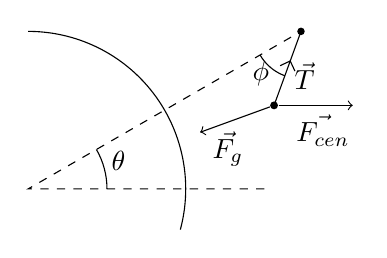
\begin{tikzpicture}[scale=2]
        \tikzset{
            patharrow/.pic={
                \draw (-0.1, -0.1) -- (0, 0) -- (-0.1, 0.1);
            }
        }
        \draw (-15:1) arc[start angle=-15, end angle=90, radius=1];
        \draw (0:0.5) arc[start angle=0, end angle=30, radius=0.5]
            node[anchor=west, pos=0.7] {$\theta$};

        \draw[dashed] (0:1.5) -- (0:0) -- (30:2);
        \draw[fill] (30:2) circle[radius=0.2mm];

        \draw (30:2) -- ++(250:0.5)
            pic[pos=0.4, rotate=70] {patharrow}
            node[pos=0.6, anchor=west] {$\vec{T}$}
            node[circle, fill, minimum size=1mm, inner sep=0] (A) {};
        \draw (30:1.7) arc[start angle=210, end angle=250, radius=0.3]
            node[anchor=east, pos=0.8] {$\phi$};

        \draw[->] (A) -- +(200:0.5)
            node[pos=0.6, anchor=north] {$\vec{F_g}$};

        \draw[->] (A) -- +(0:0.5)
            node[pos=0.6, anchor=north] {$\vec{F_{cen}}$};
    \end{tikzpicture}
    \caption{Diagram of example~\ref{exHangingString}: a hanging string}
    \label{figHangingString}
\end{figure}
\begin{example}[Hanging string]
    Consider figure~\ref{figHangingString}.
    The forces are:
    \begin{equation*}
        \vec{F_g} = -mg\uvec{r}
    \end{equation*}
    \begin{align*}
        \vec{F_{cen}} &=-m \vec{\omega} \times (\vec{\omega} \times \vec{x}) \\
        &= m\omega^2 r\cos{\theta} \left(\cos{\theta}\uvec{r} - \sin{\theta} \uvec{\theta}\right)
    \end{align*}
    If the string makes an angle $\phi$ with the radial direction,
    \begin{equation*}
        \vec{T} = T\cos{\phi}\uvec{r} + T\sin{\phi}\uvec{\theta}
    \end{equation*}
    In equilibrium, the forces must balance:
    \begin{align*}
        -mg + m\omega^2 r \cos^2\theta + T\cos{\phi} &= 0 \\
        -m\omega^2 r \cos{\theta}\sin{\theta} + T\sin{\phi} &= 0 \\
    \end{align*}
    Solving for $T$ and $\phi$:
    \begin{equation*}
        \tan{\phi} = \frac{\omega^2 r cos{\theta} \sin{\theta}}{g - \omega^2 r \cos^2{\theta}}
    \end{equation*}
    \label{exHangingString}
\end{example}
\section{Coriolis Force}
The Coriolis force is given by:
\begin{equation}
    \vec{F_{cor}} = -2m\vec{\omega} \times \vec{v}
    \label{eqnCoriolis}
\end{equation}
The force is dependent on velocity but independent of position. It has the same form as the Lorentz force, with $\vec{B} \to \vec{\omega}$, so moving particles will turn in circles.
\begin{example}[Hurricanes]
    The Coriolis force is responsible for the formation of hurricanes.\par
    Hurricanes are formed by a low-pressure region of air. Where winds blow inward toward this low-pressure zone, the Coriolis force causes the air particles to rotate and causes swirling winds around the original low-pressure zone. This effect is less near the equator, where the Coriolis force acts normal to the surface of the earth, but does not overcome gravity.
\end{example}
\end{document}